\section{Introduction}

Communication in the sciences is often done through combining the mediums of text,
data visualizations, and code. The idea of literate programming \cite{knuth84} has
been influential in providing documenting code with a large amount of context. In data
analytics this idea has been taken further, much work is done using
the popular ``notebook interface'' \cite{kluyver16}, allowing a data scientist to 
interleave code with its own results, and expository text. 

Whilst these tools are no doubt useful, they do not necessarily provide complete
transparency. Code used in notebooks is often highly abstract, providing wrappers
for complex underlying models which have often been applied as black-boxes.

A readers comprehension of such a document may be further improved by the addition of
interactive features to such visualizations. For example, in \figref{table-explanation},
whilst the text provides a summary of the table, a readers understanding can be improved
by allowing them to interact with the table itself, to see the data it summarizes,
or highlight the text underneath to see the corresponding data in the table. 

Enabling the reader to click on parts of a chart to see the data it summarizes, 
in a similar manner to the example with the table, the reader is more able to 
understand what the author of a document is trying to say.

Authoring of articles in this format is already difficult and time-consuming, and asking
the author to build in interactive features is unreasonable. Crucially, there are
no tools that treat supporting text as a visual element to interact with, and it is
not entirely clear what interactive text might look like. 

Some of the difficulty can be mitigated by building visualizations with a tool
which provides automatic support for interaction, but existing solutions do
not come with the ability to extend these visualizations with supporting text.
As a body of text, a scientific article is full of references to the topic of
discourse, meaning a large number of interactive elements which would be labourious to manually
link to visualization elements. Thus any tool that helps solve this problem will need an automated
component.

\begin{figure}[h]
   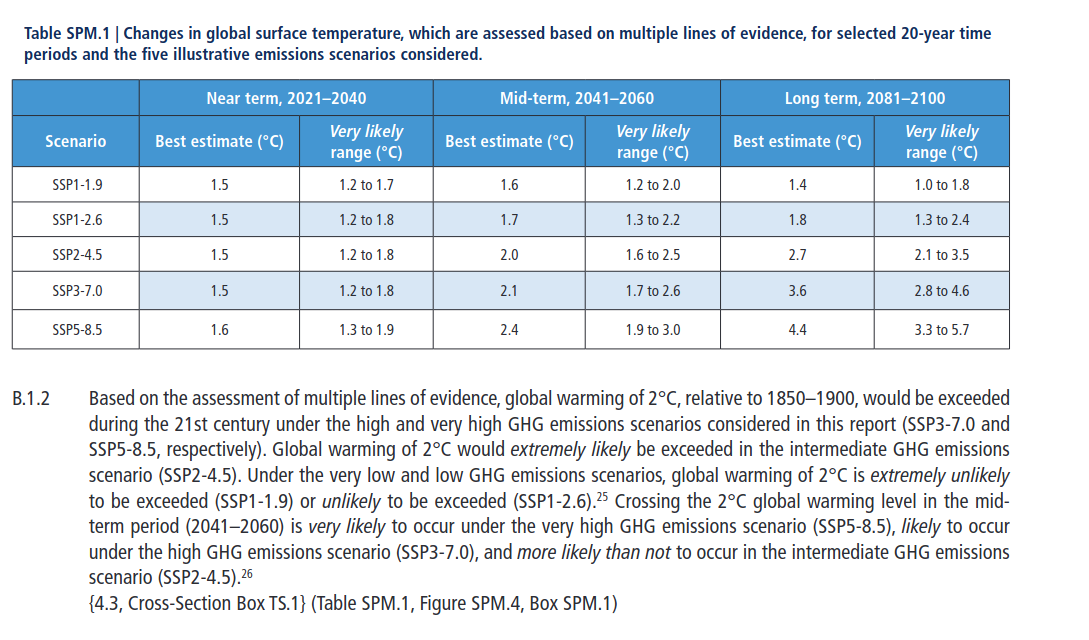
\includegraphics[width=0.7\textwidth]{fig/ipcc-table-explanation.png}
   \caption{Explanation based on the contents of a table}
   \label{fig:table-explanation}
\end{figure}